You will need to add a couple of hardware components to your Cow Pi circuit before you can start this lab.

\subsection{Necessary Components}

Figure~\ref{fig:components-mk4b} shows the components you will need for the range finder and alarm.

\begin{figure}
    \centering
    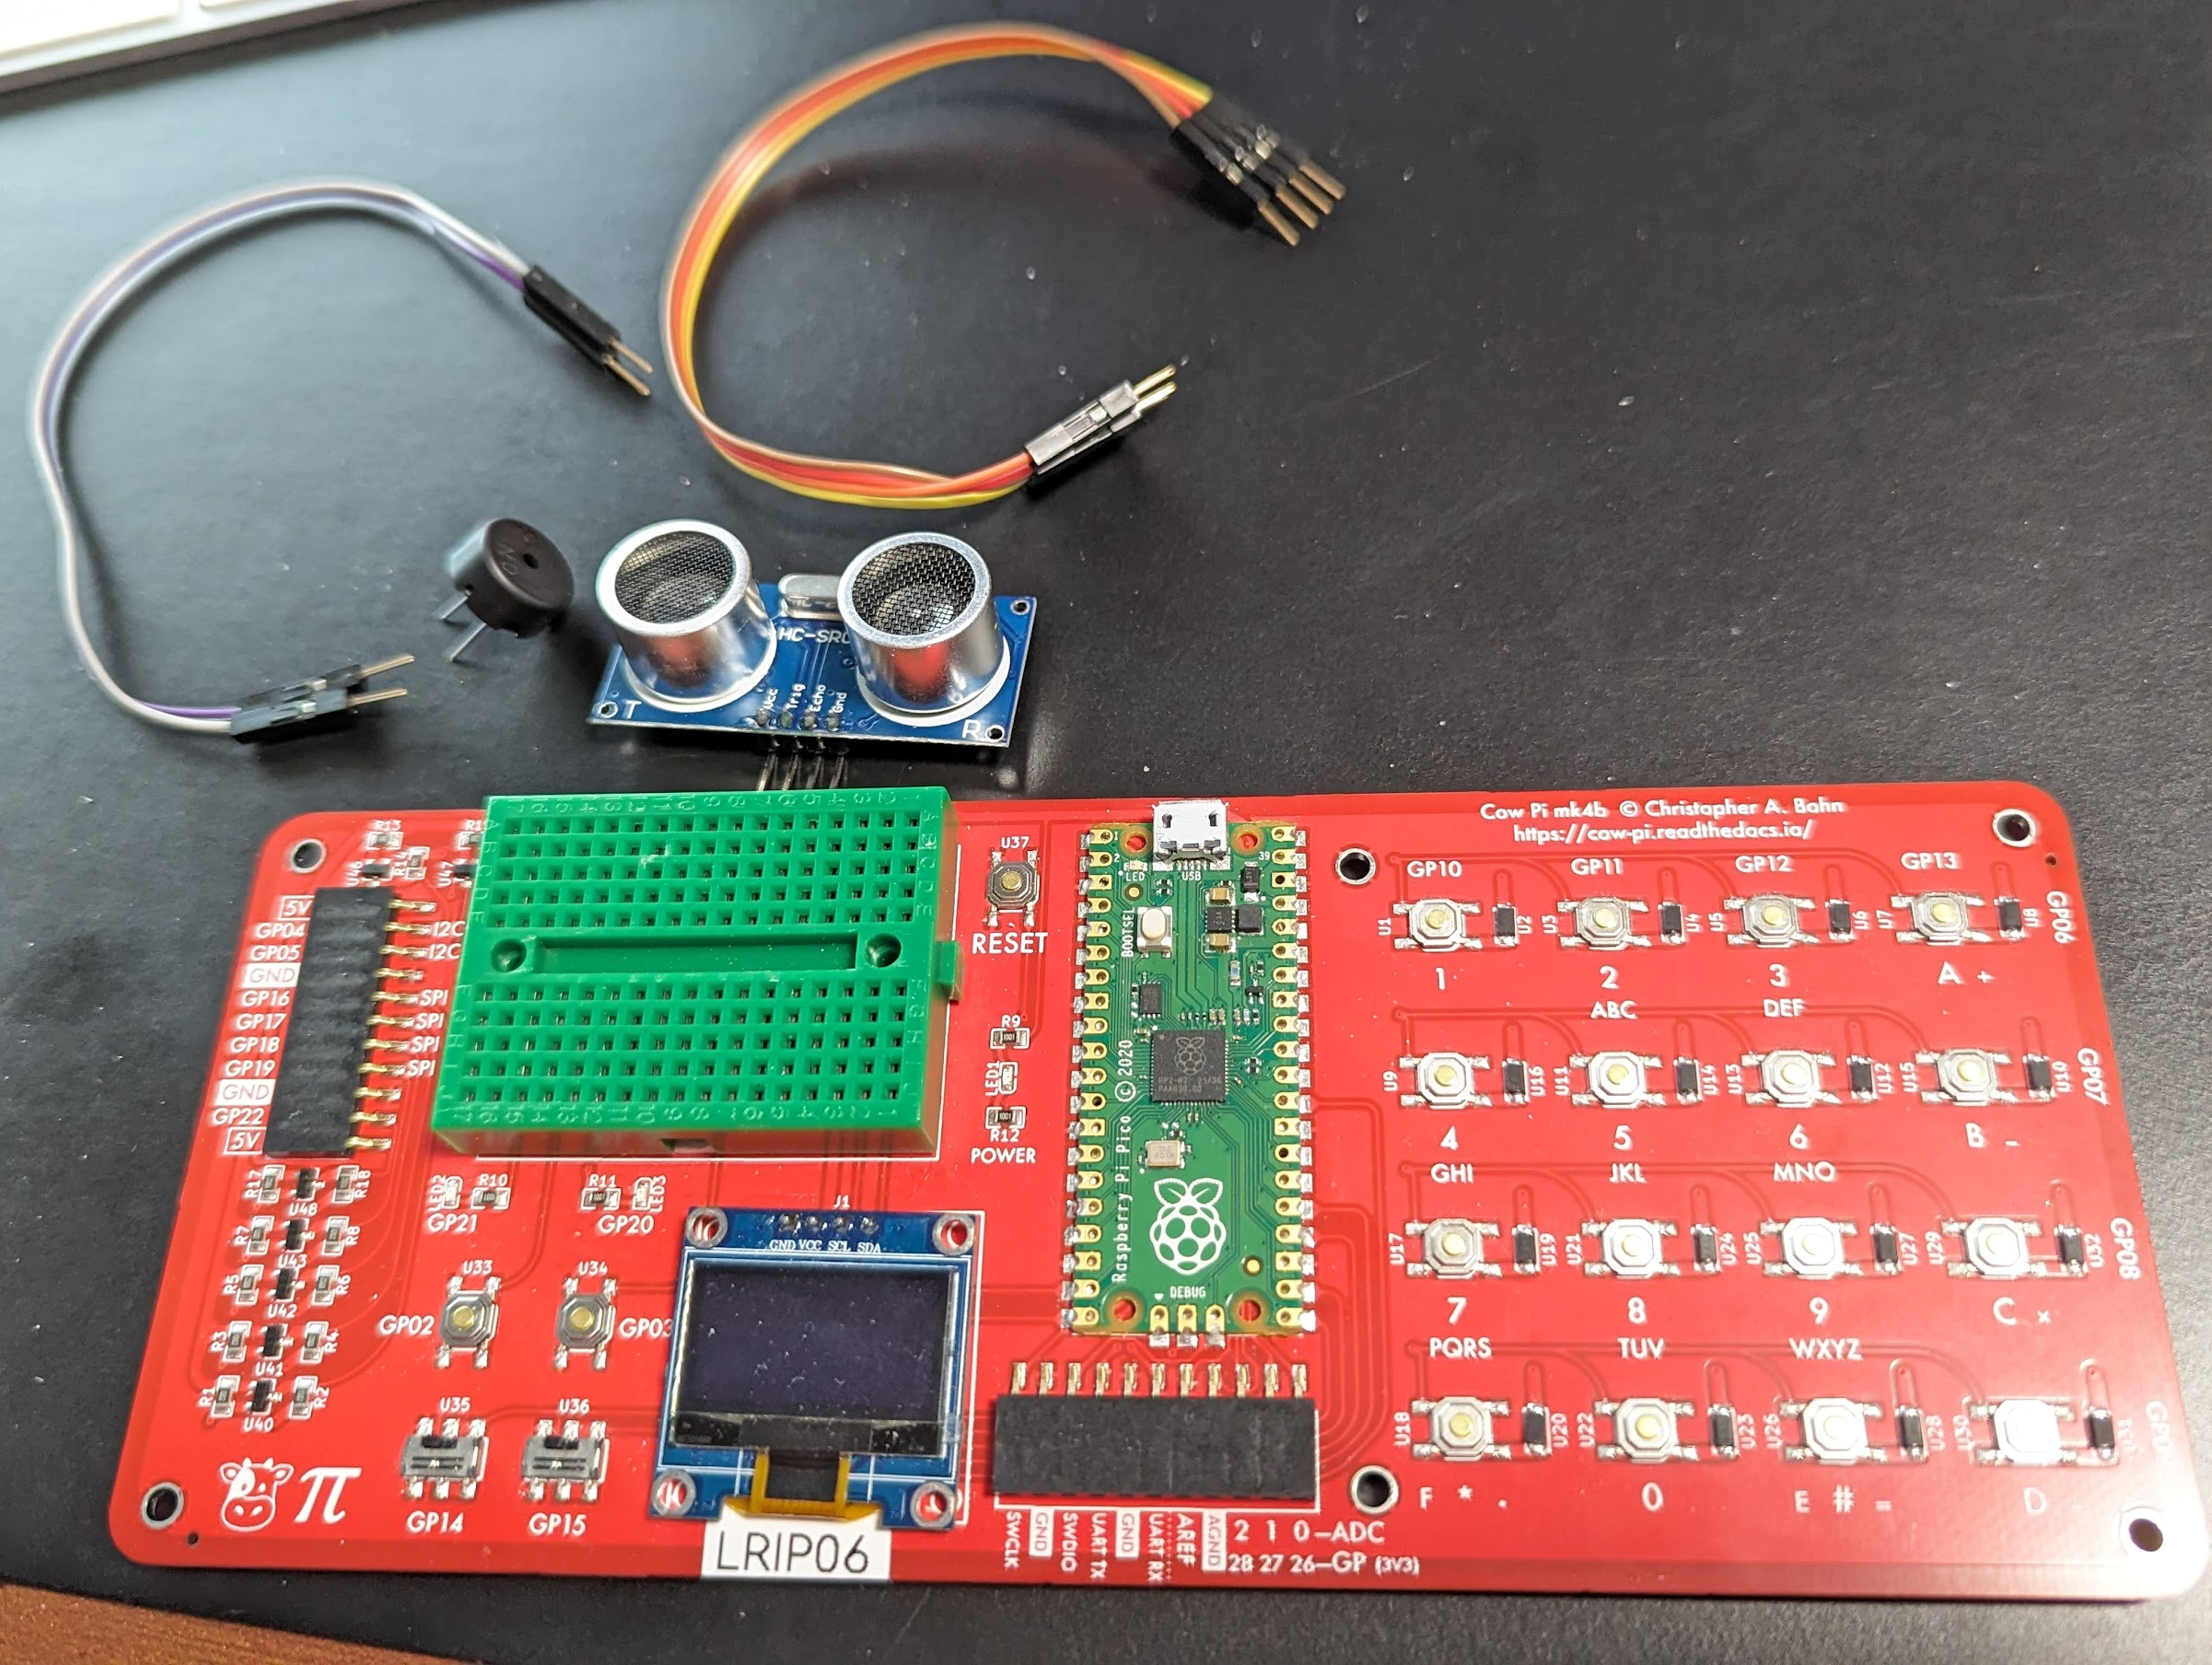
\includegraphics[width=10cm]{hardware/mk4b/components} % TODO: change to mk4b
    \caption{Components needed for the Range Finder \label{fig:components-mk4b}}
\end{figure}

You will need:
\begin{itemize}
    \item Your Cow Pi hardware circuit
    \item A piezoelectric ``passive buzzer''
    \begin{itemize}
        \item Piezoelectric devices can convert electric energy into mechanical energy, and vice-versa
        \item You will use a piezoelectric device to create an audible alarm
    \end{itemize}
    \item An ultrasonic echo sensor
    \begin{itemize}
        \item \textcolor{red}{If your sensor is still in the red bubblewrap packaging, there are also two resistors in the packaging. We will not use these, but we might have a use for them in a future semester. Please place them in the Cow~Pi's storage box.}
        \item The two prominent drums on this device are ultrasonic transducers, one of which converts electricity to 40kHz sound (well above the range of human hearing), and the other of which converts 40kHz sound into electricity
        \item You will measure the time between the ultrasound being transmitted and its reflecting being received to determine the distance to whatever is reflecting the ultrasound
    \end{itemize}
    \item Six 20cm male-to-male wires (you can separate these wires from a multi-wire cable)
\end{itemize}

There is a labeled header on the left side of the Cow~Pi;
we will use this to connect the hardware components to the RP2040 microcontroller.

\subsection{The Mini-Breadboard on the Cow Pi}

A key feature of solderless breadboards, such as the mini-breadboard on your Cow~Pi, are the groups of 5 holes (Figure~\ref{fig:breadboard-mk4b}).
Each group of five is a \textit{terminal strip}.

\begin{figure}
    \centering
    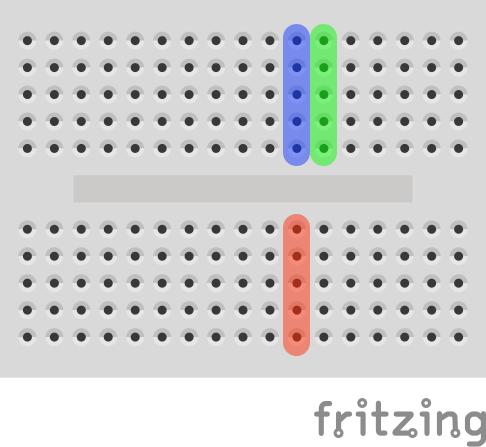
\includegraphics[height=4cm]{hardware/mk4b/breadboard}
    \caption{Terminal strips on a mini-breadboard \label{fig:breadboard-mk4b}}
\end{figure}

The five holes in a terminal strip are electrically connected to each other but are electrically isolated from the other terminal strips.\footnote{
    They are isolated for DC signals, and parasitic reactance is negligible for AC signals below about 10~kHz.
}
For example, in Figure~\ref{fig:breadboard-mk4b}, all holes in the terminal strip that is highlighted in blue are connected to each other,
but they are not connected to the holes in the adjacent terminal strip highlighted in green.
Similarly, they are not connected to the holes in the red terminal strip on the other side of the gutter.

A consequence of this is that any components' connectors that are inserted into a terminal strip are connected to the connectors of other components that are inserted into the same terminal strip.

If you want to learn more, a very good overview of solderless breadboards can be found here: \url{https://learn.adafruit.com/breadboards-for-beginners?view=all}

Figure~\ref{fig:breadboard-with-components-mk4b} shows where you will insert the hardware components for the group project.
(The precise placement is not critical, so long as you make a note of which terminal strips you use.)

\begin{figure}
    \centering
    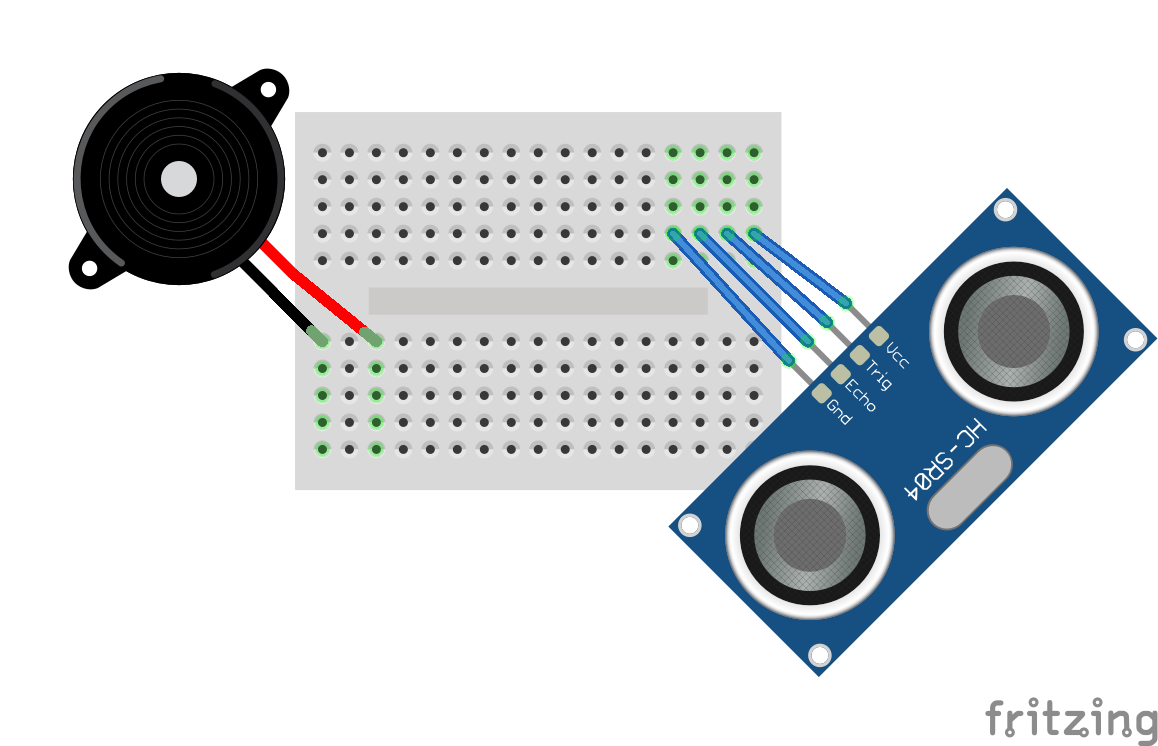
\includegraphics[height=4cm]{hardware/mk4b/breadboard-with-components}
    \caption{Terminal strips on a mini-breadboard \label{fig:breadboard-with-components-mk4b}}
\end{figure}


\subsection{Connecting the ultrasonic echo sensor}

Take a look at the ultrasonic echo sensor (Figure~\ref{fig:ultrasonic-mk1f}).
Notice that it has four pins, labeled \texttt{Gnd}, \texttt{Echo}, \texttt{Trig}, and \texttt{Vcc}.

\begin{figure}
    \centering
    \subfloat[The back side of the ultrasonic sensor.]{
        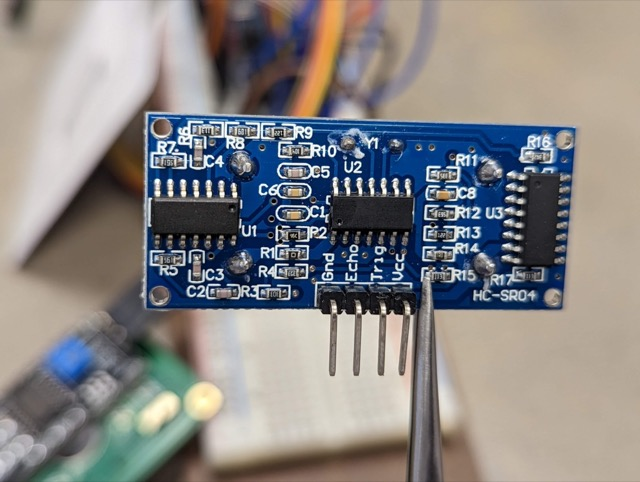
\includegraphics[height=4cm]{hardware/components/ultrasonic_rear}
%        \label{fig:ultrasonicRear}
    }
    \hfil
    \subfloat[The front side of the ultrasonic sensor.]{
        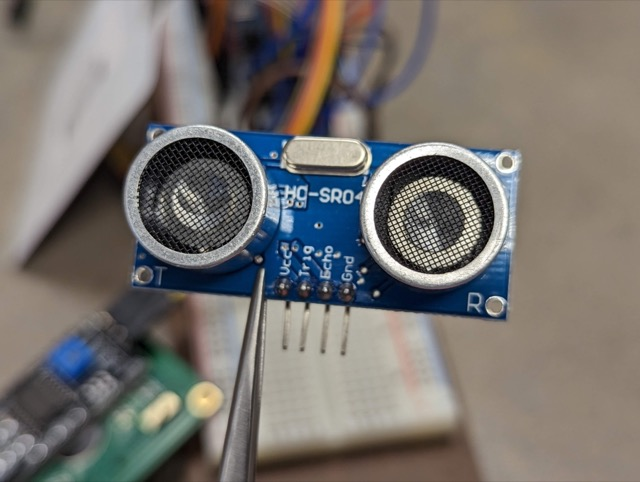
\includegraphics[height=4cm]{hardware/components/ultrasonic_front}
%        \label{fig:ultrasonicFront}
    } \\
    \subfloat[Inserting the ultrasonic sensor.]{
        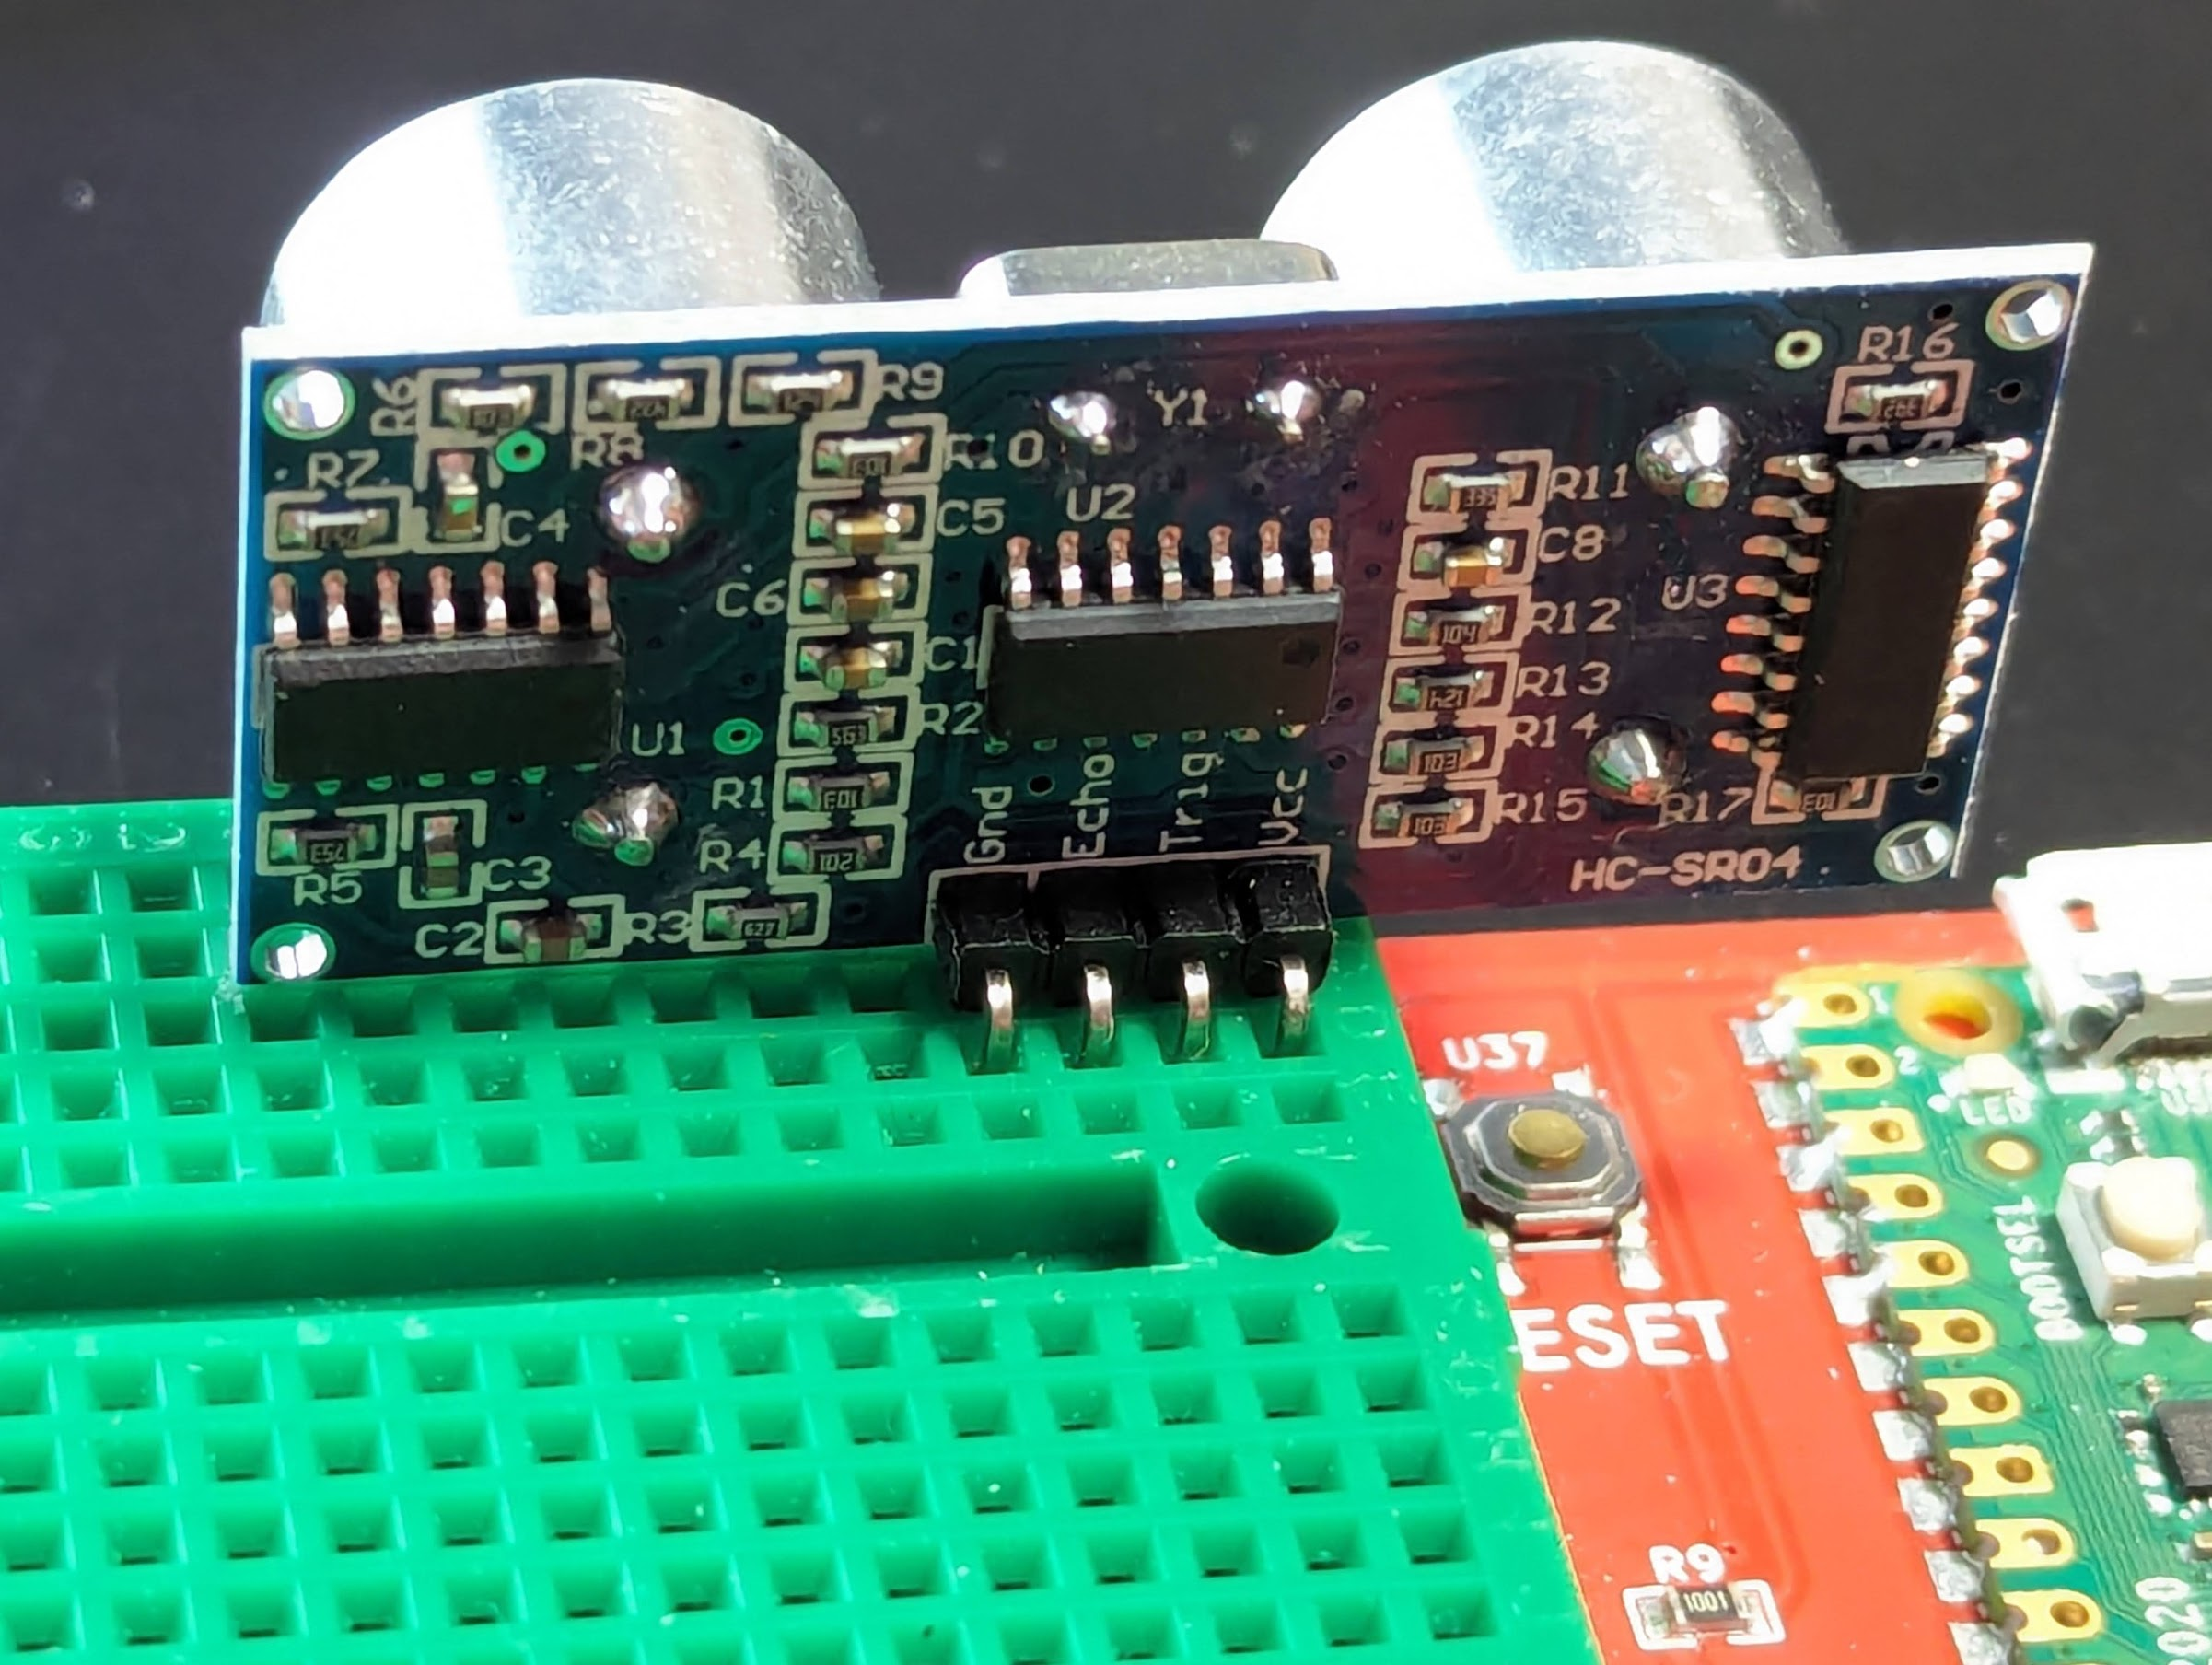
\includegraphics[height=4cm]{hardware/mk4b/insert-ultrasonic}
    } \\
    \subfloat[One end of the board's connection to the sensor.]{
        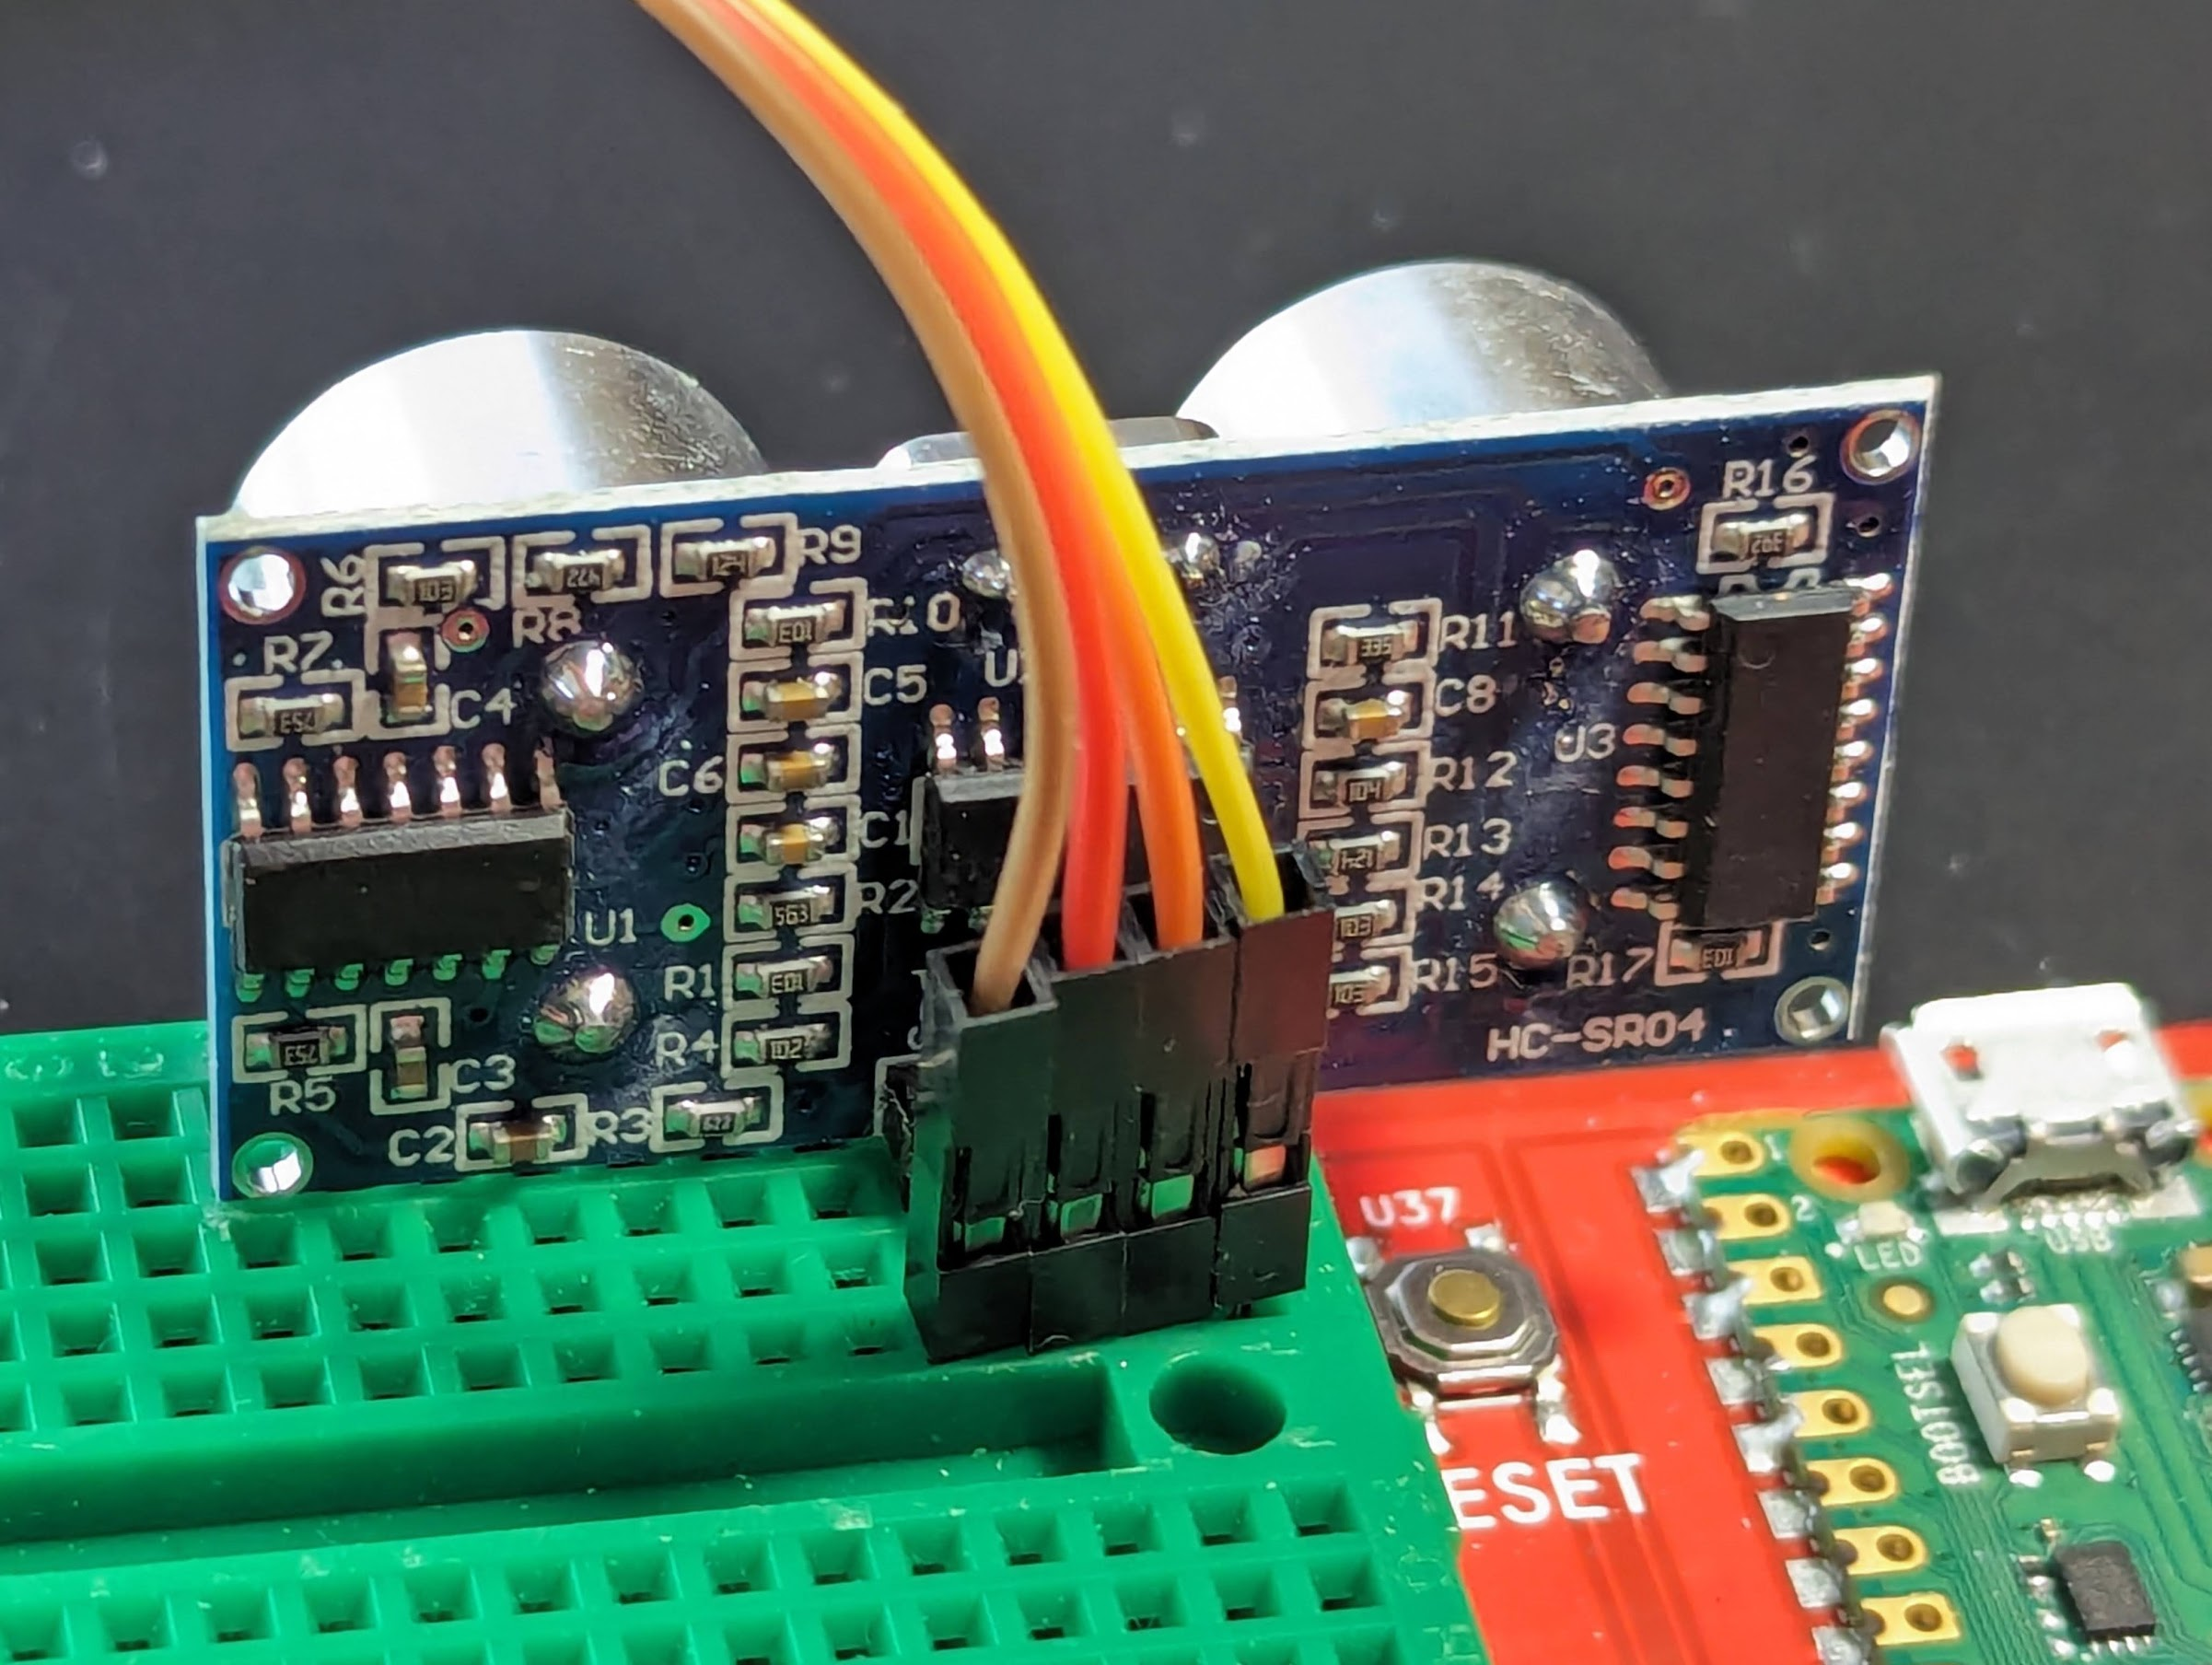
\includegraphics[height=4cm]{hardware/mk4b/connect-ultrasonic-1}
    }
    \hfil
    \subfloat[The other end of the board's connection to the sensor.]{
        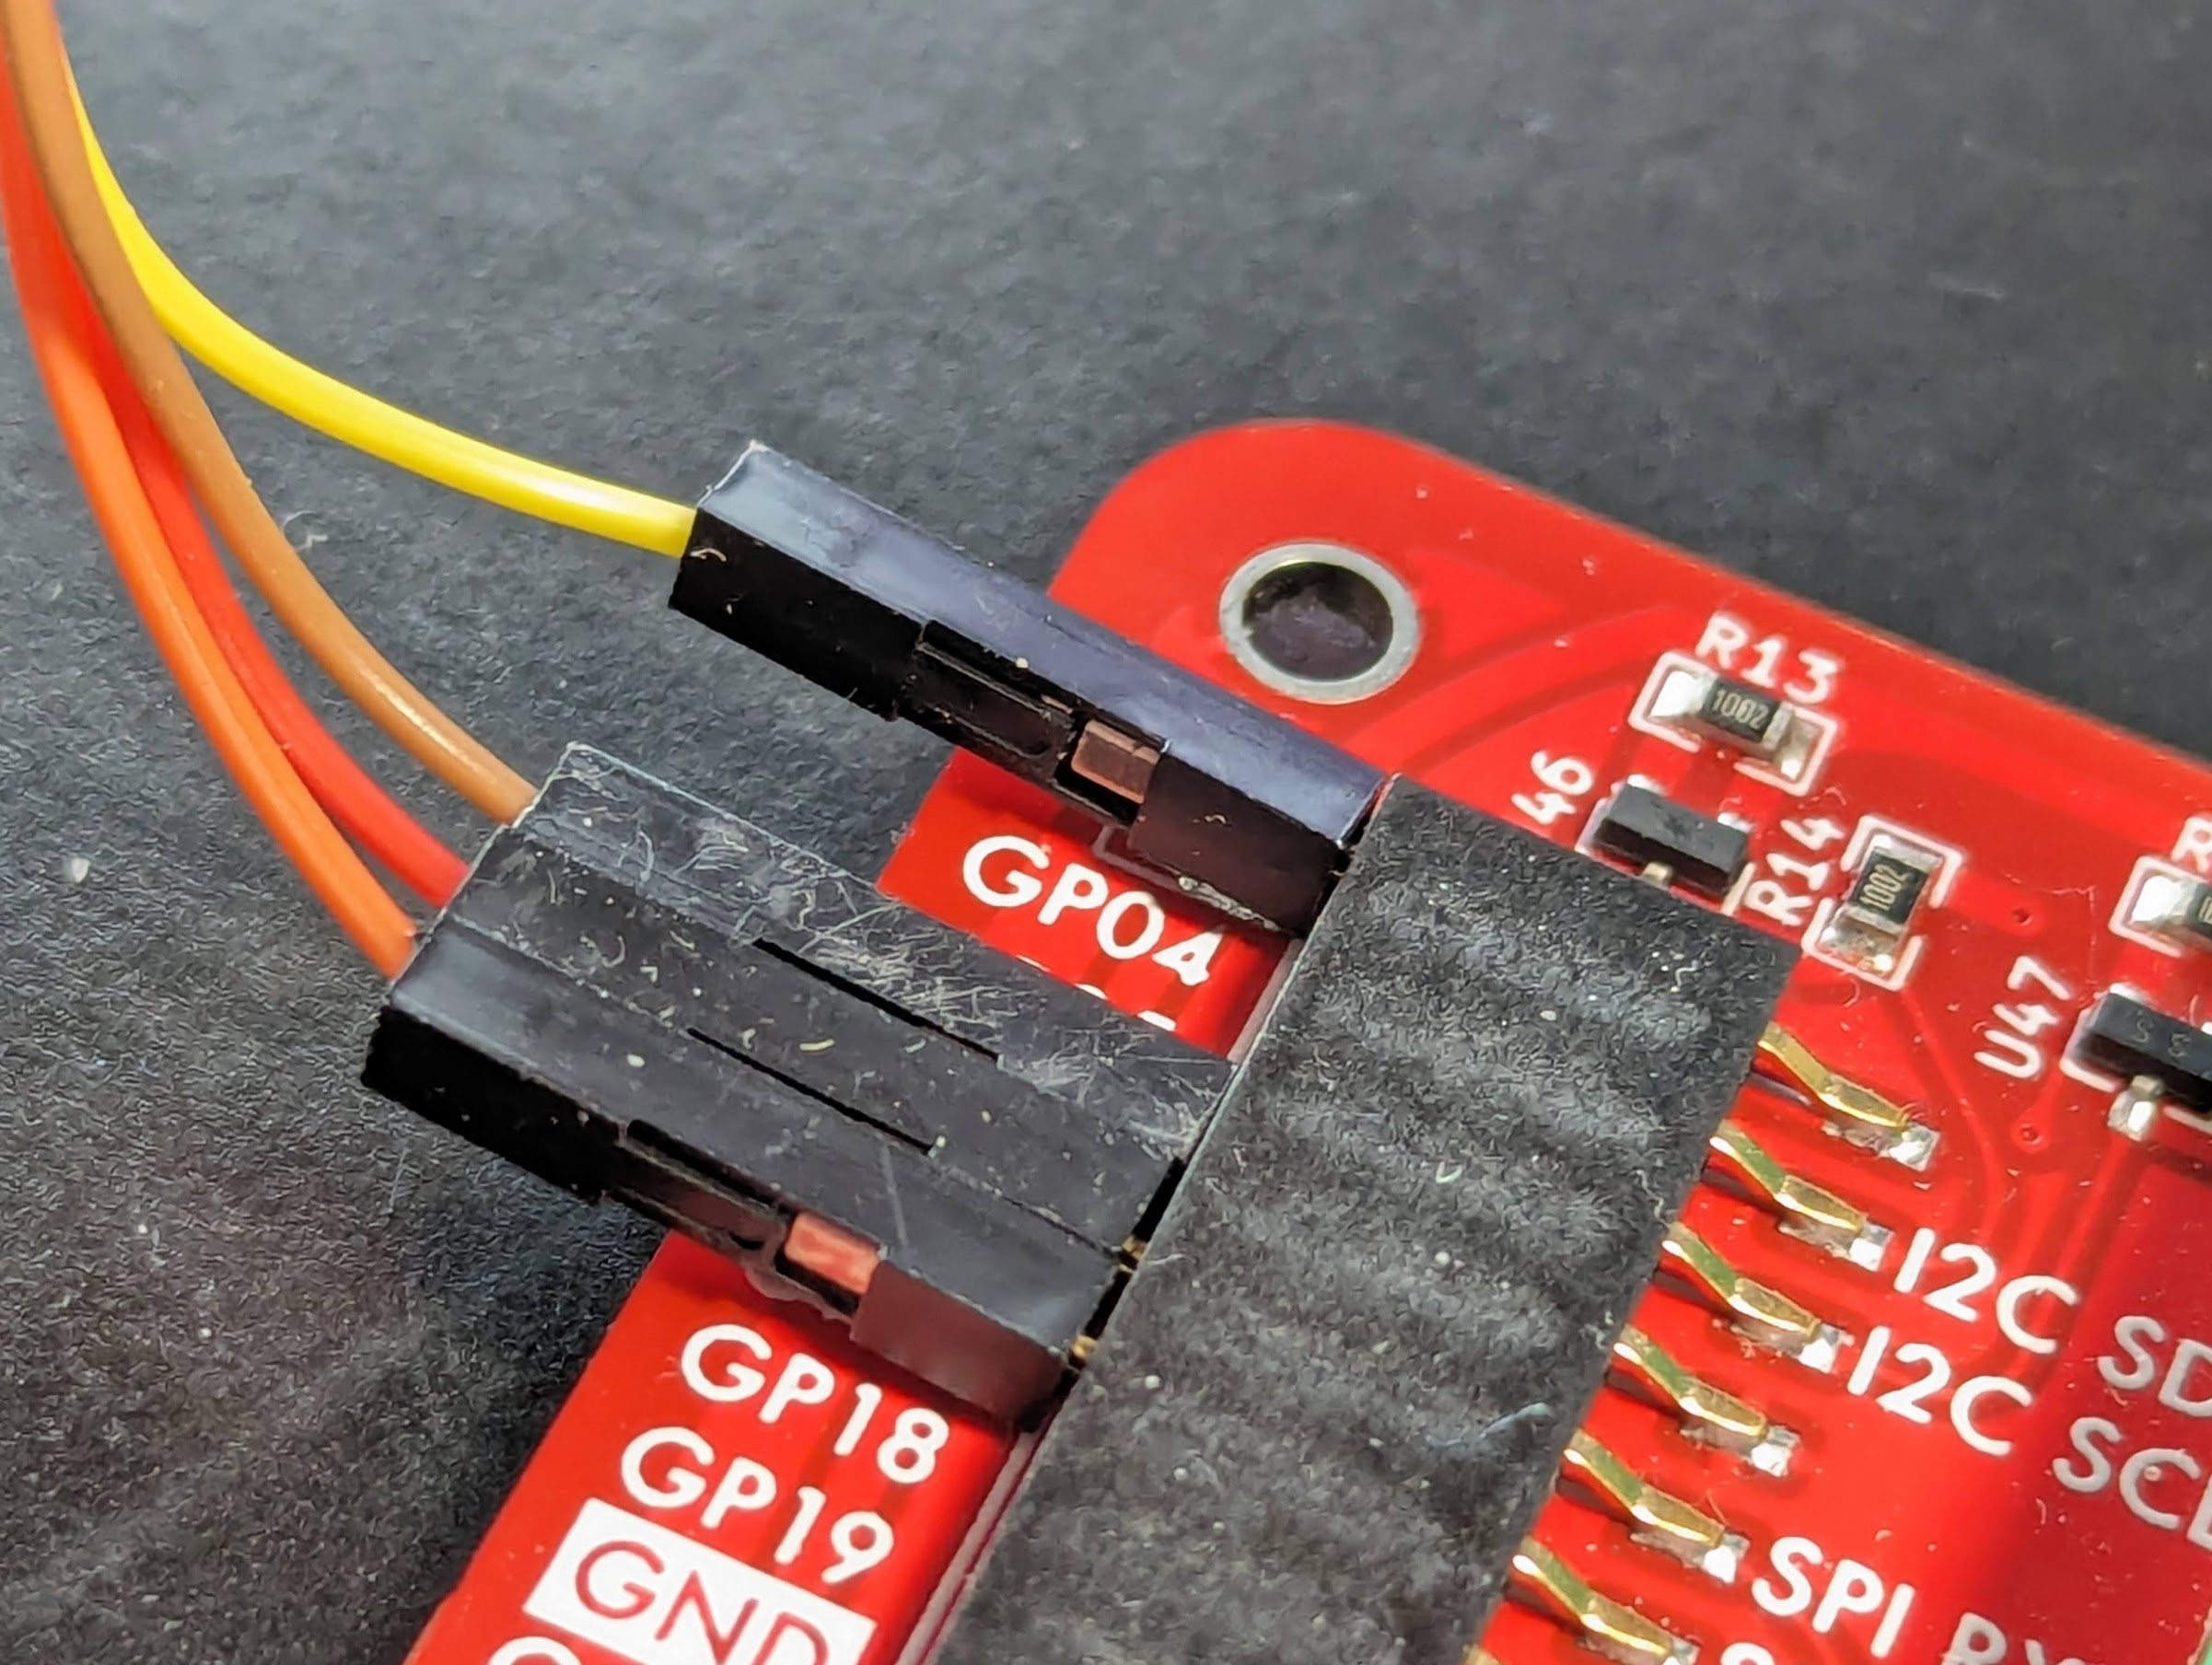
\includegraphics[height=4cm]{hardware/mk4b/connect-ultrasonic-2}
    }
    \caption{The ultrasonic echo sensor. \label{fig:ultrasonic-mk4b}}
\end{figure}

\begin{description}
    \checkoffitem{Insert the ultrasonic echo sensor into unused rows on the breadboard, pointing away from you.
        Leave room behind the sensor to connect a wire into each of the same terminal strips that the sensor uses.}
    \checkoffitem{Insert four 20cm wires, one into each of the same terminal strips that the sensor uses.
        Make a note of which color wire corresponds to which of the sensor's pins.}
    \checkoffitem{Insert the other end of the \texttt{Vcc} wire into a \texttt{5V} slot}
    \checkoffitem{Insert the other end of the \texttt{Gnd} wire into a \texttt{GND} slot}
    \checkoffitem{Insert the other end of the \texttt{Echo} wire into the \texttt{GP16} slot}
    \checkoffitem{Insert the other end of the \texttt{Trig} wire into the \texttt{GP17} slot}
\end{description}

The ultrasonic echo sensor is now connected to the Raspberry Pi Pico's pins \texttt{GP16}--\texttt{GP17}.
The starter code will configure \texttt{GP17} (\lstinline{TRIGGER}) to be an output pin and \texttt{GP16} (\lstinline{ECHO}) to be an input pin.


\subsection{Connecting the Piezobuzzer}

\begin{figure}
    \centering
    \subfloat[Inserting the piezobuzzer]{
        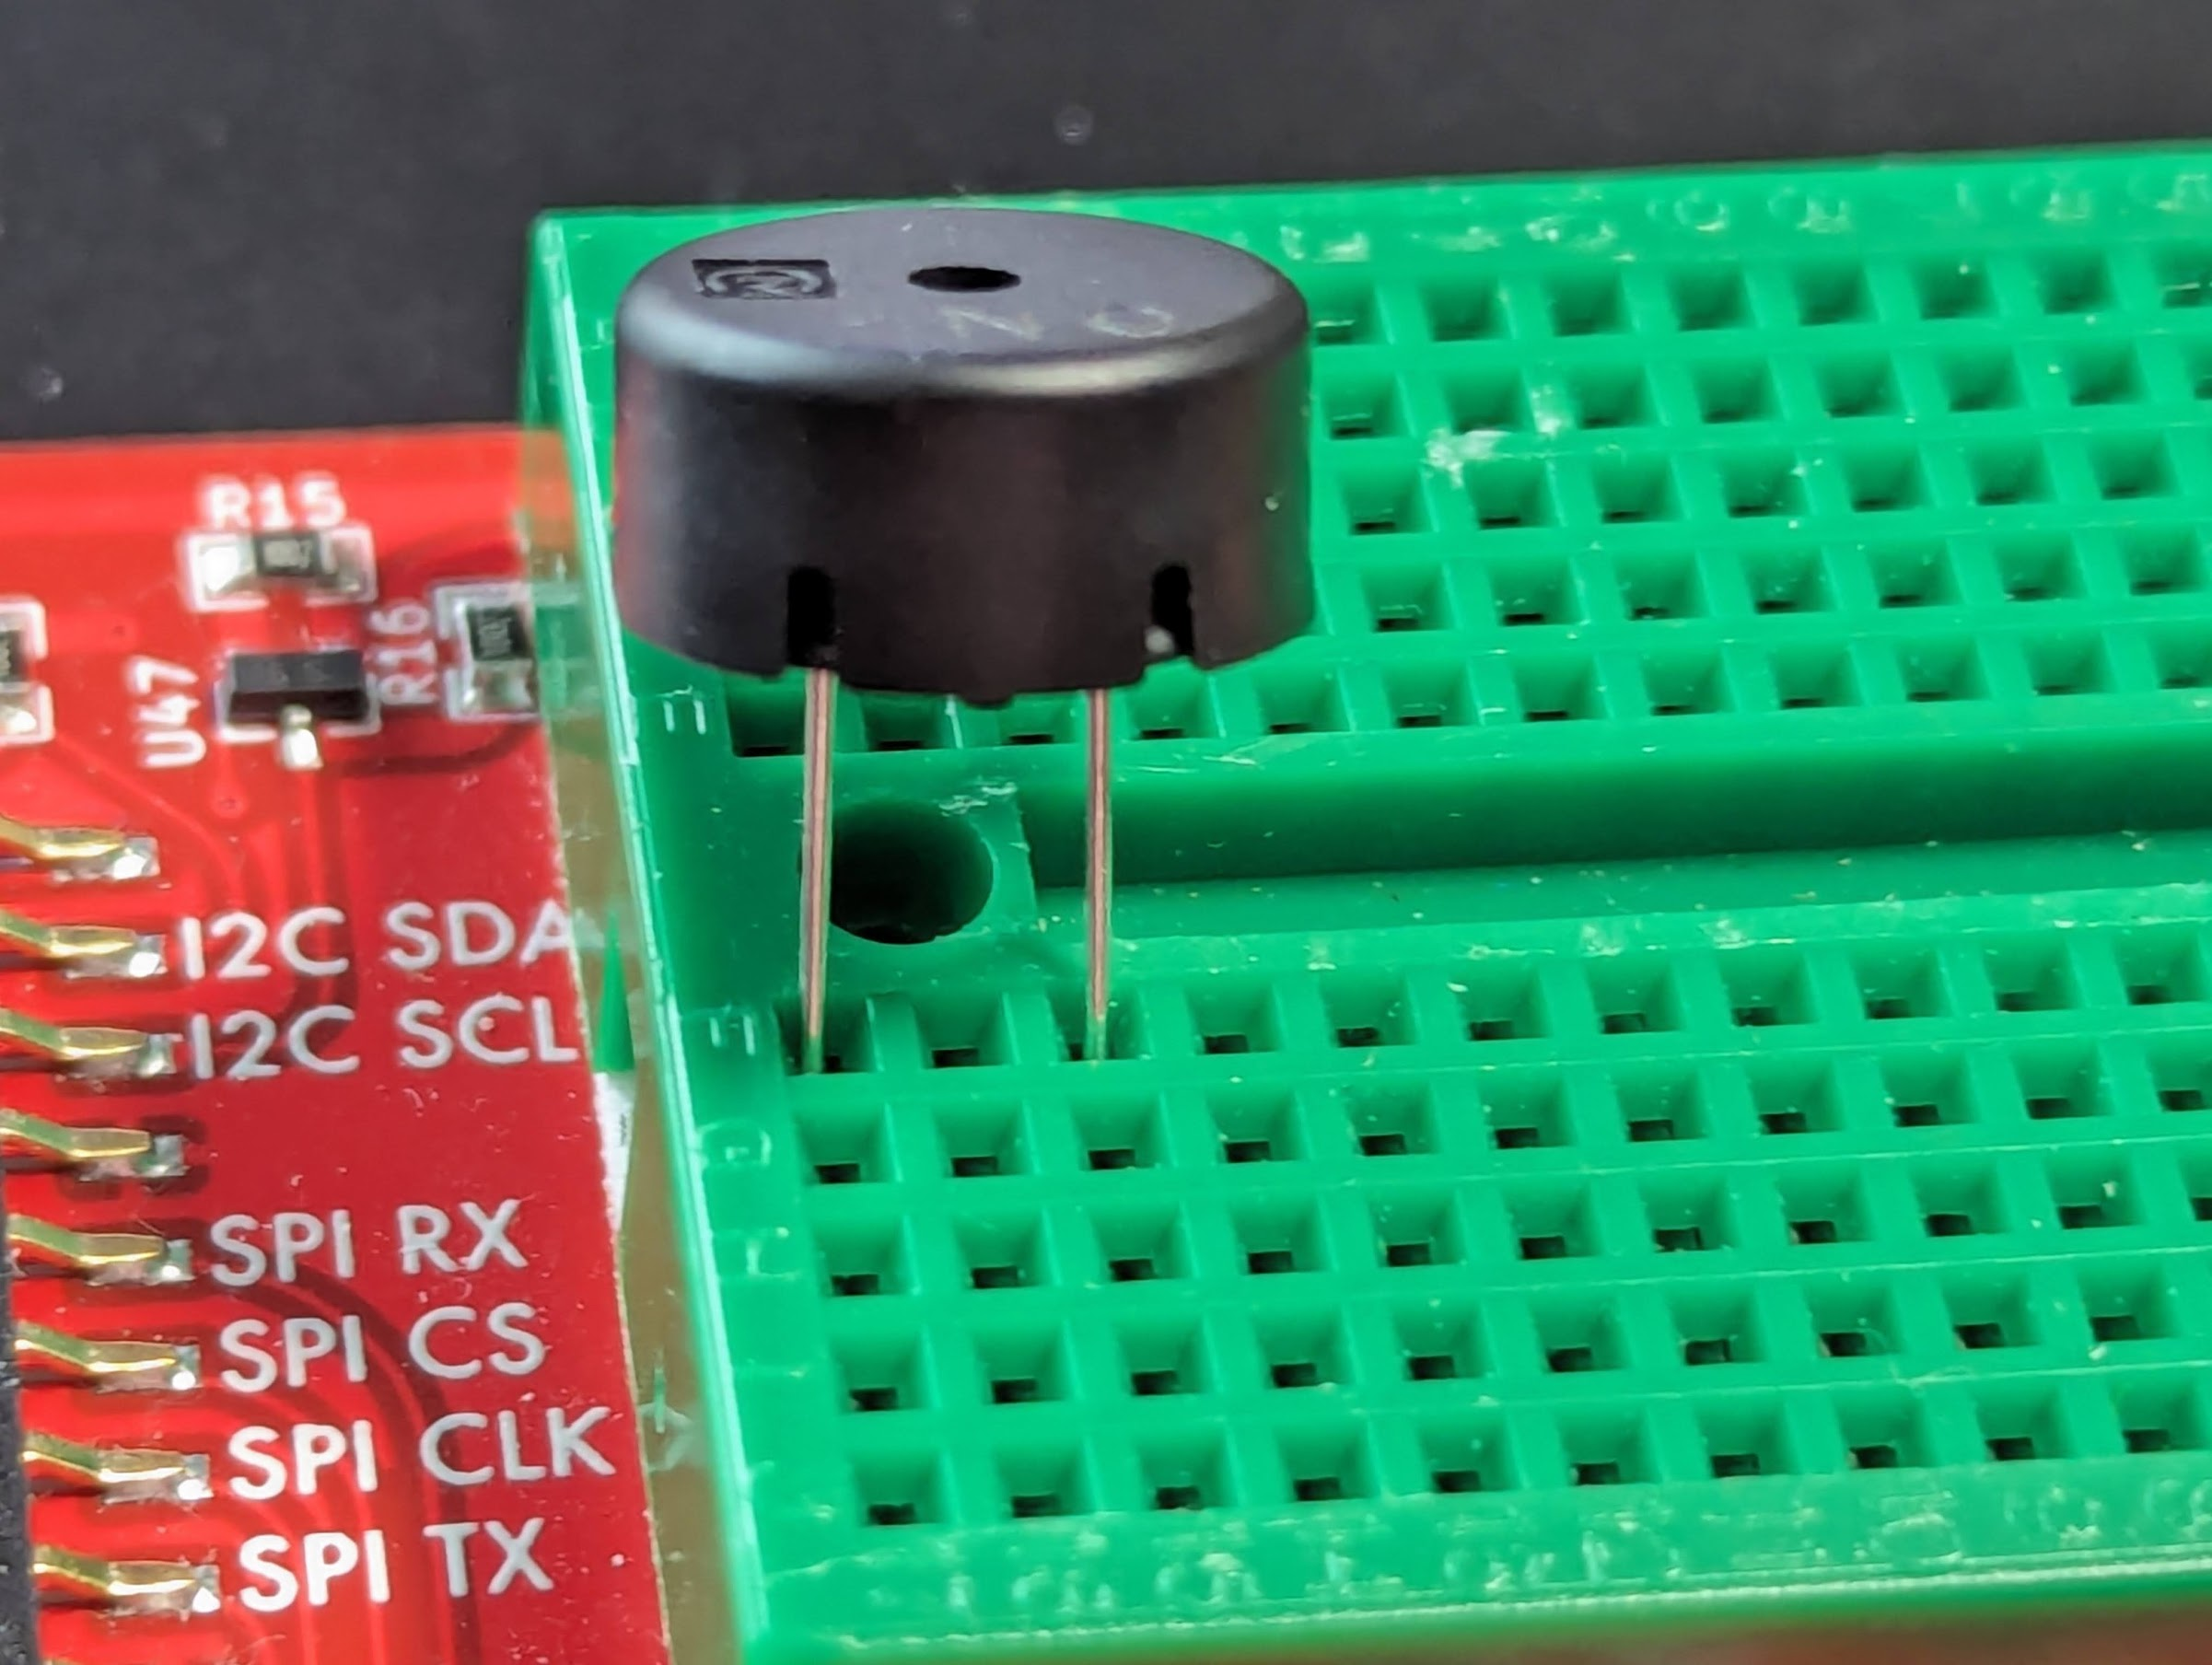
\includegraphics[height=4cm]{hardware/mk4b/insert-piezo}
    }
    \hfil
    \subfloat[The front side of the ultrasonic sensor.]{
        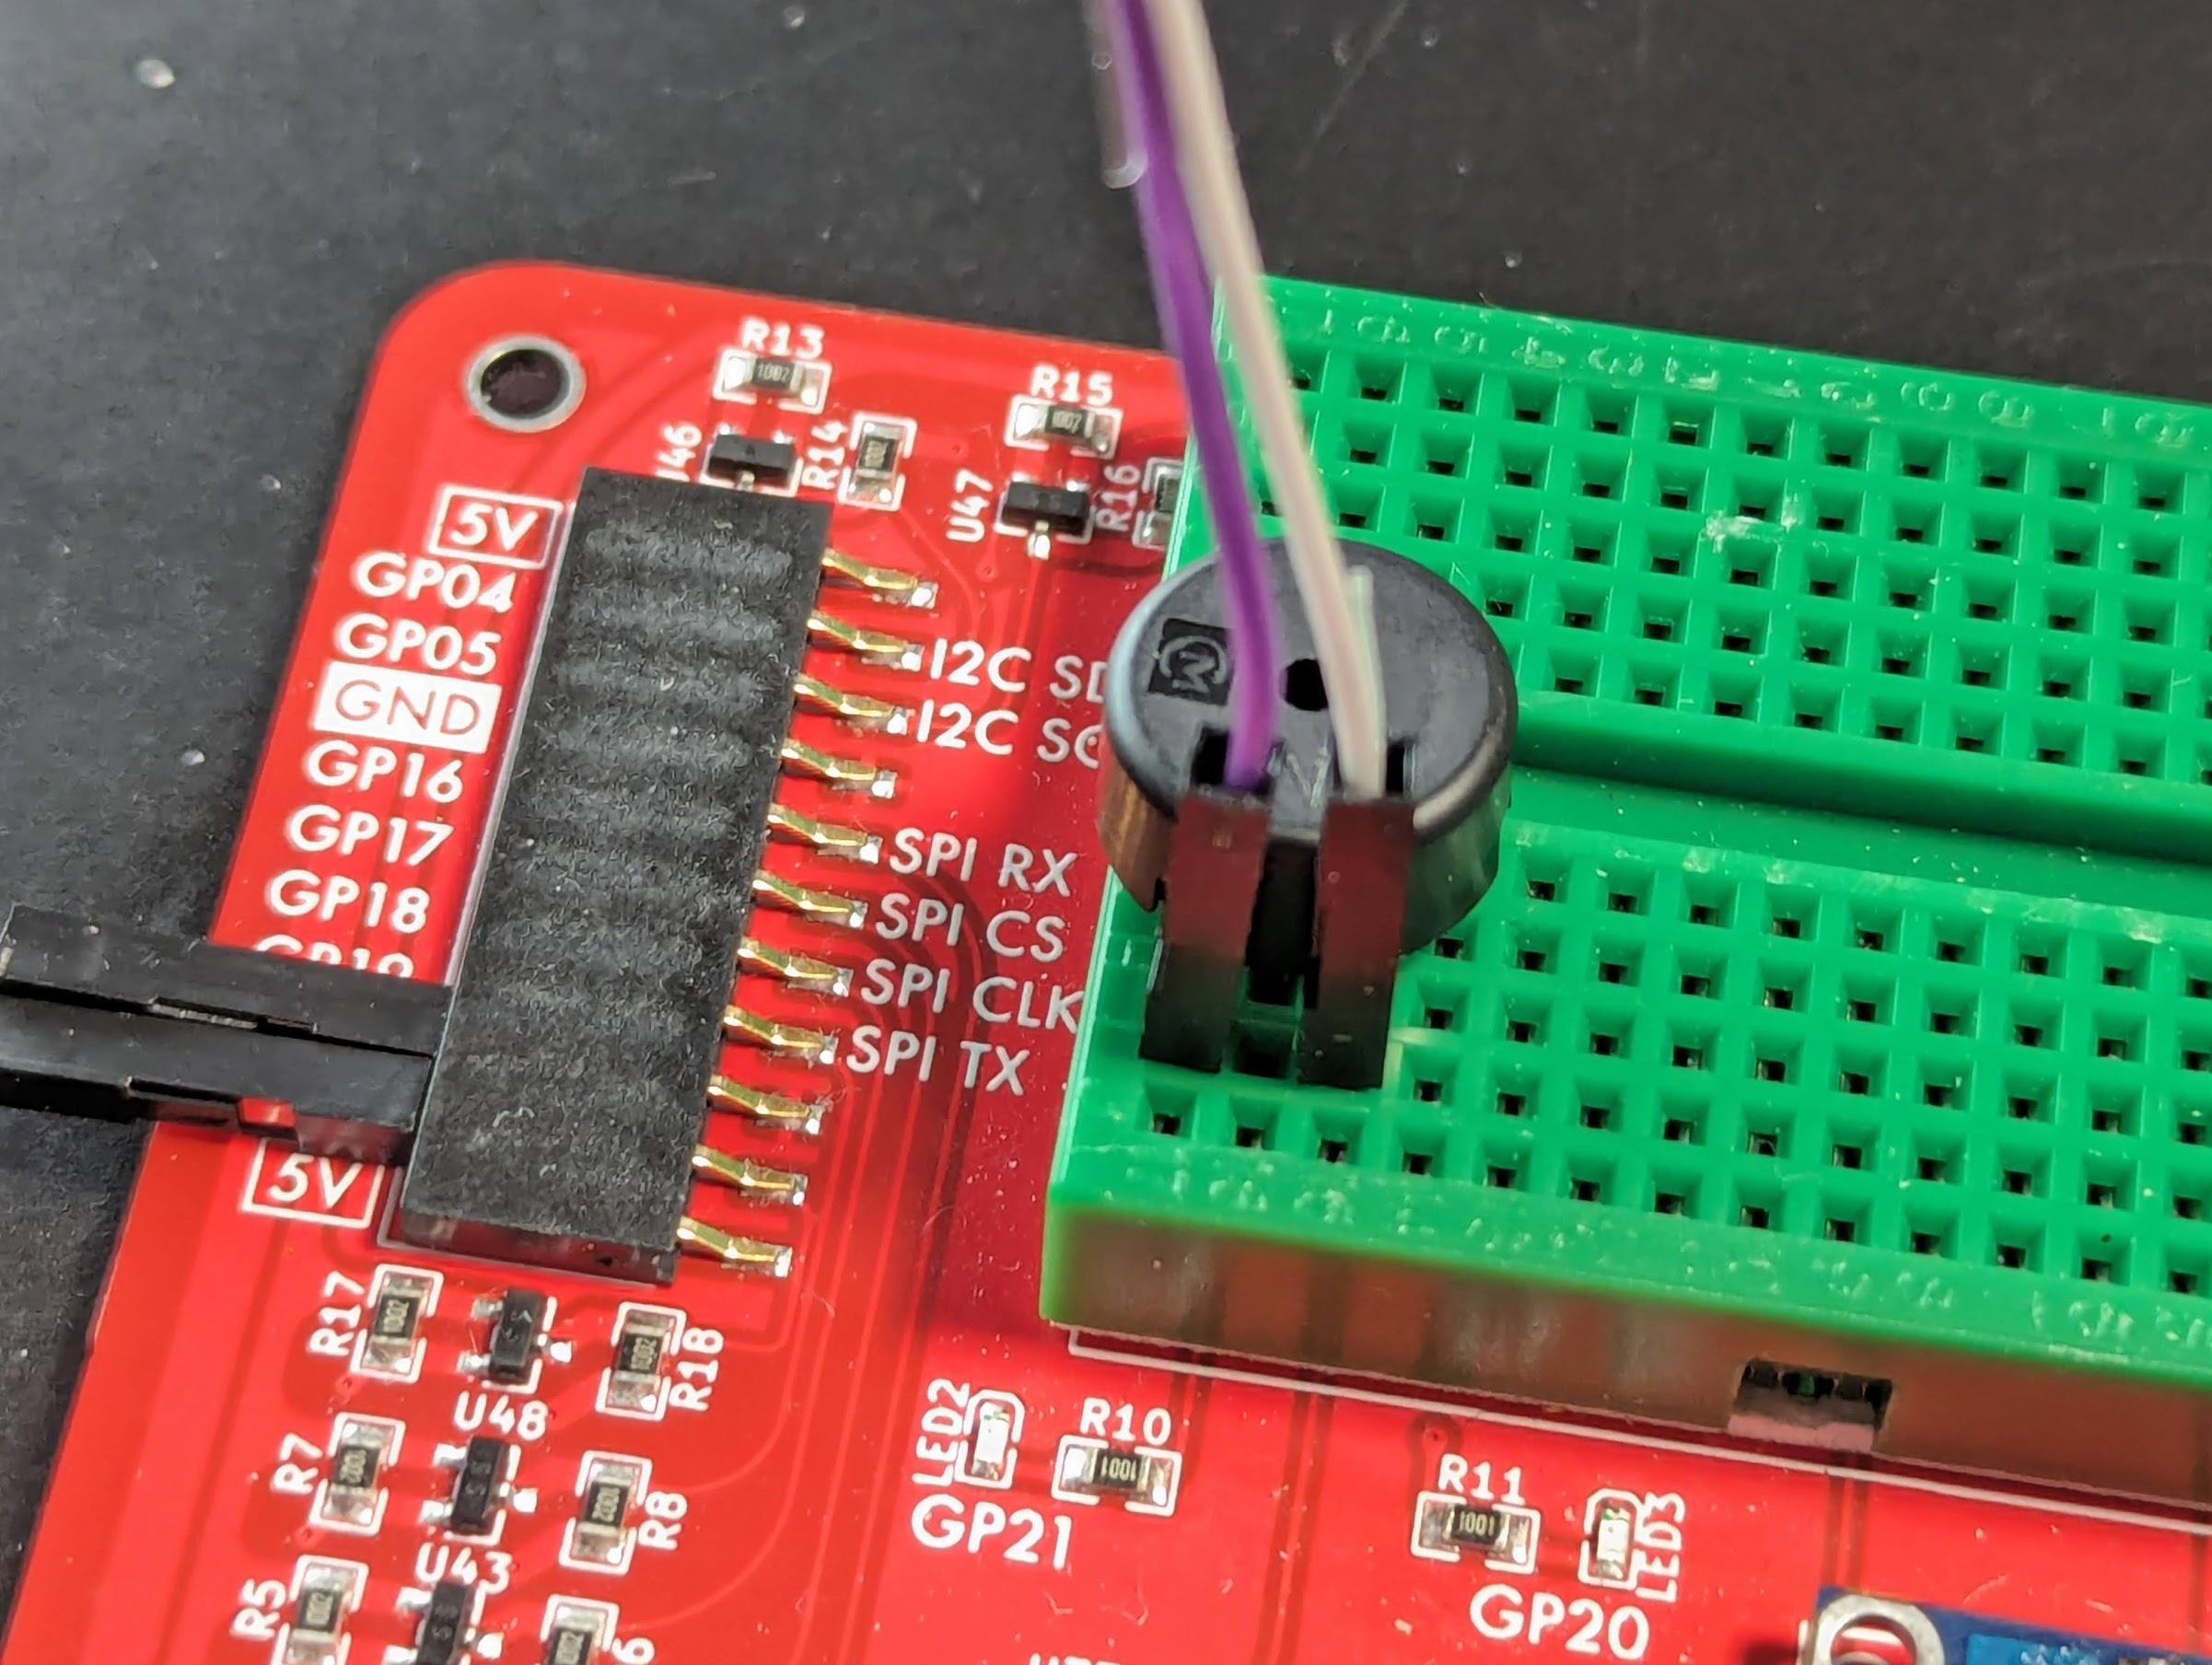
\includegraphics[height=4cm]{hardware/mk4b/connect-piezo}
    }
    \caption{The piezoelectric ``passive buzzer''. \label{fig:piezobuzzer-mk4b}}
\end{figure}

\begin{description}
    \checkoffitem{Insert the piezobuzzer into unused rows on the breadboard.
        Leave room to connect a wire into each of the same terminal strips that the piezobuzzer.}
    \checkoffitem{Insert two 20cm wires, one into each of the same terminal strips that the piezobuzzer uses.}
    \checkoffitem{Insert the other end of one of the wires into a \texttt{GND} slot
        \begin{itemize}
            \item For \textit{this} particular device, the polarity does not matter, so it doesn't matter which wire is connected to \texttt{GND}
        \end{itemize}}
    \checkoffitem{Insert the other end of the other wire into the \texttt{GP22} slot}
\end{description}

The piezodisc can now be operated through the Raspberry Pi Pico's pin \texttt{GP22}.
The starter code will configure \texttt{GP22} (\lstinline{BUZZER}) to be an output pin.


\vspace{1cm}

Your Cow~Pi is now ready for you to design and code the software for a range finder and alarm.
